\chapter{系统设计}
\label{cha:design}

\section{总体结构}
\label{chap3:structure}

\subsection{系统设计目标}
\label{sec:goal}

为了满足第~\ref{sec:requirements}节中描述的需求,该系统的主要设计目标是:

\begin{itemize}
    \item 可以从互联网设备搜索引擎API中获得主机系列(域名、IP地址、IP地址段等)的信息,
    如IP地址、操作系统信息(操作系统名称、发行版及版本号)、地区信息(国家、地区、城市等)、
    服务器信息(服务器框架名称及版本号)、软件信息(软件名称及版本号)等;
    \item 可以对主机信息进行信息融合,对相同主机的信息进行合并,对不同主机的信息进行再次搜索后合并;
    对同一台主机的不同数据源的信息进行合并时,不同字段的数据进行合并;
    \item 可以从CVE相关网站上获得CVE名称列表,并用爬虫对CVE的信息进行数据爬取,
    获得CVE的名称、描述、CVSS\cite{mell2007complete}(通用漏洞评分系统)分数、产生威胁的端口、
    产生威胁的软件信息(软件名称、版本号、制造商、软件类型等)、相关网页等;
    \item 可以对主机信息和CVE信息进行对比分析,如端口信息、软件信息等,找出可能产生的威胁;
    \item 可以把从API和网站上获取的主机信息、CVE信息和可能的威胁情报信息存储到数据库中,并在需要的时候进行读取;
    \item 可以由用户设置监测的主机的范围(域名、IP地址、IP地址段等),定时更新主机信息、CVE信息,
    并重新分析可能的威胁情报,如一天、一星期甚至一个月;
    \item 每次发现新的威胁情报之后,通知事先设置好的邮箱或者其他联系方式,该次分析发现了哪些威胁信息;
    \item 提供一个前端,可以直观地看到设置的主机系列的主机上有哪些主机存在威胁,
    并且尽可能提供威胁的原因,也能直观地观察该主机的全部信息,如采用列表等;
    \item 在可能的威胁情报过多时,前端提供过滤功能,可以搜索某一特定CVE,
    系统返回可能受到该CVE威胁的主机列表;也可以搜索某一特定IP地址(用户想监测的主机范围内的),
    系统返回这个IP是否受到某些CVE的威胁,如果不存在威胁的话就不会看到结果;也可以搜索某一主机的范围(域名、IP地址段等),
    系统返回有关这个范围的主机的威胁情报信息;
    \item 当在发现主机上存在威胁时,从一些特定网站上获得该漏洞的检测脚本,在前端上显示。
\end{itemize}

\subsection{系统工作流程}
\label{sec:process}

图~\ref{fig:main-process}是系统的工作流程图。
\begin{figure}[H]
    \centering
    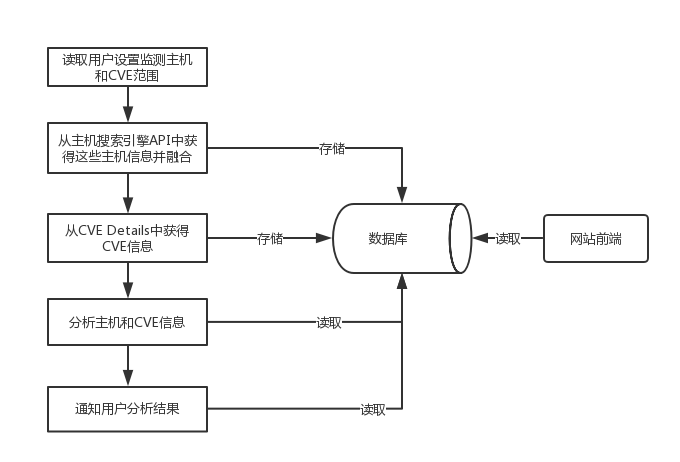
\includegraphics[scale=0.6]{main-process}
    \caption{系统总体工作流程图}
    \label{fig:main-process}
  \end{figure}
可以看出,在每次更新时,首先读取用户设置的监测主机和CVE的范围,其中主机范围可以是IP地址段(如:166.111.0.0/16)、
域名(如:tsinghua.edu.cn),或者IP地址(如:166.111.176.55);CVE的范围可以使全部、某些年的,或者某些指定的CVE。

接着,系统从互联网设备搜索引擎API中获得与这些主机范围相关的主机的信息,这些信息会返回许多台主机的信息,
然后由系统应用合并的算法对这些信息进行合并融合,最后返回一个主机信息的并集。这些主机信息的并集存储在数据库中以备之后的使用,
这些信息将会在分析威胁情报和显示前端的时候进行读取。

下一步是进行CVE信息的获取,在第一步中已经获得了需要监测的CVE的范围,因此这里只对这些CVE进行数据的爬取。
这里采用的是爬虫的方法,对网站CVE Details进行网页页面的解析,获得其中的有用信息,并将这些信息存储在数据库中,
这些信息将会在分析威胁情报和显示前端的时候进行读取。

接下来由系统读取之前的主机信息和CVE信息并对信息进行比对,通过主机的信息,如开放端口、
安装软件等Fingerprint来判断任意一台主机是否有可能受到某些CVE的威胁。如果有,则将这台主机的可能受到威胁的信息存储到数据库中,
如CVE名称、CVE描述、相关信息(References)、可能受到威胁的原因等。这些信息将会在推送和显示前端时进行读取。

分析完威胁情报,系统将会对这些威胁情报进行推送。用户可以在一开始设置主机范围和CVE范围的文件中设置希望收到推送的邮箱,
也可以同时设置重点关注的CVE名称。在这一步中,系统将会把本次分析的全部结果,和每个用户关注的CVE的分析结果发送给这些邮箱。

最后还有一个环节是网页前端,这个前端是对存储了主机信息、CVE信息和威胁情报信息的数据库的一个直观的表示。
在前端中,用户可以看到每一台主机的可能受到威胁的CVE的信息,如果需要,也可以看到原始的主机信息,也可以进行更高级的搜索,
如:搜索IP地址、IP地址段、域名、CVE名称等。

\section{网络主机信息获取设计}
\label{chap3:hosts-design}

\subsection{互联网设备搜索引擎API介绍}
\label{sec:API-intro}

在相关工作中已经介绍过互联网设备搜索引擎的功能,它们会扫描整个互联网,
而用户可以通过一些关键词来找到自己想要的互联网设备的有关资源配置和部署信息的报告。
而所谓这些搜索引擎的API就是这些网站的开发者开放给其他开发者的一套提供和网站基本相同功能的API,开发者可以通过这些API开发自己的软件。

而本系统最重要的一个步骤就是对主机信息进行融合,而这些信息的来源不是来自主动的扫描,
而是来自这些搜索引擎的API,这些API的信息又有所不同(这也是本文工作意义的主要原因之一),
因此对这些API进行各自提供的信息的对比将是进行主机信息获取前的第一步。本文进行信息融合选取的API是Censys、Shodan和ZoomEye,
因此在下文中主要对这三种API进行对比分析。

\subsection{Censys API}
\label{sec:Censys-API}

Censys提供了一套REST API和Python中相应的模块,可以通过搜索关键词进行主机信息的获取,
如IP地址、IP地址段、域名等,还可以自定义一些字段的值,
如在搜索“80.http.get.status\_code: 200”时将会搜索HTTP协议开放80端口的GET的返回值为200的主机,
同时,Censys还提供了布尔表达式、范围(Range)搜索、正则表达式搜索等诸多功能。Censys的API文档如下:https://censys.io/api。

不过,对于一个API,最关注的内容还是其提供的信息内容。我们主要关注的Censys的API有两个,
一个是/search,一个是/view。/search可以通过关键词搜索信息,Censys会返回一个列表给用户,
每一个结果的字段由用户指定,关键词的语法如上文所述,支持主机IP地址(/search/ipv4)、
网站(/search/websites)和证书(/search/certificates),这里主要关注的是主机;
/view是在用户已经明确知道主机的IP地址或者域名之后,可以查看该主机的完整信息,同样支持IP地址(/view/ipv4)、
网站(/view/websites)和证书(/view/certificates),这里主要关注的是主机。在使用/search搜索的时候,
需要哪些字段需要用户指定,如果不指定Censys只会给每个结果返回一些摘要信息,而这些信息是不够用的。因此,往往需要结合上述两个API来使用。

不论是搜索还是详情的API,Censys返回给用户的主要是运行在这台主机上的开放端口上的服务的Fingerprint信息,
如运行在80端口上HTTP服务的GET请求的返回值、状态值、文件头等;还有如运行在22端口上的SSH服务的密钥交换的参数、加密算法等。
不过,对于需要自动化的融合工作来说,这就需要对每一种协议做分别处理,因为对于每一种协议,Censys返回的数据的结构是不同的,
如果不能有效地提取需要的信息,就是没有意义的。为了更加有效地使用Censys,本文仅用/search来获得更多的IP地址,
因为相比另外两个API,Censys返回的结果条数往往都更多,但是对于其返回的Fingerprint信息,则仅取其端口信息和运行的操作系统信息。

此外,在校园网环境下Censys的访问速度较慢,往往需要10秒钟以上的时间来返回一次查询,而且如果需要大量的查询次数的话需要付费。

\subsection{Shodan API}
\label{sec:Shodan-API}

Shodan同样提供了一套REST API和Python中的模块,也相应地提供了自己的语法,比如搜索“net:166.111.0.0/16”搜索网段信息等。
Shodan的API文档如下:https://developer.shodan.io/api。

而对于Shodan返回的信息,它的格式要更加地统一。我们关注的API主要有两个,一个是/host,类似于Censys的/view,
可以查看一台主机的全部详细信息;一个是/search,和Censys的/search类似,也支持自己的语法。在/host返回的结果中,
Shodan会返回一些基本信息,这些和Censys是类似的,如地理位置、ASN、组织、ISP等等,更重要的是它提供的各种服务的Fingerprint信息更加格式化,
在“data”字段中,Shodan提供了运行在其上能找到的所有服务的信息,
而把协议名称、传输层协议、运行的软件名称及版本、对应域名等都用相同的字段的名字存储,在自动化处理的时候十分方便。
类似地,/search的结果也只给每个条目一部分基本信息,比如“data”字段只返回了第一个服务的结果,
因此同样需要结合/host使用。此外值得一提的是,在每一种服务里面,Shodan还提供了本机可能受到威胁的CVE的列表,
这和本文想做的工作本质上是一样的,只是本文将扩充这个列表,从其他数据源获取数据,然后与这个列表求并集。

此外,速度方面,Shodan访问比Censys快。返回结果数方面,结果条数比Censys少不少。权限方面,可以免费申请教育账号,获得更高访问权限。

\subsection{ZoomEye API}
\label{sec:ZoomEye-API}

ZoomEye同样提供了一套REST API和Python中的模块,但是提供的数据要更少,不过其中也有另外二者没有的结果条目。不过,和前两者不一样的是,
ZoomEye没有提供类似于/view或者/host类似的API,只能一次搜索一系列的主机,并在结果里直接返回主机的相关信息。
ZoomEye的API文档如下:https://www.zoomeye.org/api。

我们主要关注的ZoomEye的API有/host/search和/web/search,它们都是通过搜索ZoomEye自己的一套语法之后返回一系列主机,
然后这两个API分别返回主机上的基本信息(地理位置、开放端口、操作系统等)和Web应用信息(应用、容器、框架、防火墙等)。
因为本文的对比方法主要是通过主机上的应用和可能受到CVE威胁的软件进行对比得到结果,所以实际使用中使用了/web/search这个API。

此外,ZoomEye的访问速度也较快,但是返回的结果只返回其中的30\%,条数比较少。

\subsection{各API对比表格}
\label{sec:API-comparation-table}

综合以上三小节的内容,表~\ref{tab:API-comparation}是这三个API的对比分析表格。

\begin{table}[htb]
    \centering
    \begin{minipage}[t]{0.8\linewidth}
    \caption{Censys,Shodan,ZoomEye API对比}
    \label{tab:API-comparation}
      \begin{tabularx}{\linewidth}{XXXX}
        \toprule[1.5pt]
        {\heiti 对比项} & {\heiti Censys} & {\heiti Shodan} & {\heiti ZoomEye} \\\midrule[1pt]
        访问速度 & 慢 & 快 & 快 \\ 
        结果数目 & 多 & 一般 & 少 \\
        支持语法 & 支持 & 支持 & 支持 \\
        选用API & /search/ipv4 & /search, /host & /web/search \\
        主要内容 & 指纹信息 & 指纹信息 & 安装软件信息 \\
        格式化 & 较复杂 & 较规则 & 较规则 \\
        特殊信息 & 详细指纹信息 & 可能的威胁 & 软件信息分类 \\ 
        权限 & 250次/月 & 学生账号不限 & 只返回30\% \\
        \bottomrule[1.5pt]
      \end{tabularx}
    \end{minipage}
  \end{table}

\subsection{主机信息获取策略}
\label{sec:hosts-strategy}

结合以上分析,本文获得主机信息的方法是从互联网设备搜索引擎的API中搜索,对于每种目标(一种目标为一个关键词,关键词为IP地址、IP地址段或者域名),
对于不同类型的目标,对每种API分别采用不同的搜索语法,对结果应用融合,然后把结果存储到数据库。

具体地,为了获得尽可能多的主机上的软件信息、服务信息和基本信息,本文对于三种API,主要使用Censys获得更多的主机地址,
仅使用/search/ipv4来搜索满足关键词条件的主机列表;用Shodan来提供详细的指纹信息,首先使用/search来获取满足条件的主机列表,
然后用/host获取每一台主机上的详细指纹信息;用ZoomEye来提供更加丰富的软件信息和版本,
仅使用/web/search来获取满足关键词条件的主机列表中主机上的软件信息。

\section{CVE信息抓取的设计}
\label{sec:CVE-strategy}

为了分析每一台主机可能受到的威胁,把主机和有固定编号的CVE进行联系,就需要每一个CVE的相关信息。和第~\ref{sec:CVE}节中提到的一样,
CVE Details就是这样一个记录了每一个CVE的详细信息的网站,也处于实时更新中。对于每一个CVE单独的界面,
它提供了该CVE的名称、简介、CVSS分数、威胁类型、可能受到威胁的软件信息、一些相关阅读等。

因为本文采用的判断是否有受到威胁的可能的方法是对比主机上安装的软件和可能受到CVE威胁的软件,和开放端口和可能受到威胁的端口,
所以在抓取CVE信息时,安装软件的信息和可能的端口信息就是必不可少的。然而,因为比对软件名称和版本号的时候无法进行精确的比对,
因为软件名称可能有多个叫法,软件版本也存在细小的差别,比如Beta版本等,仅仅进行模式匹配往往是不够的,因此,在发现可能的威胁的时候,
具体的判断最终往往还是由人来进行,这就需要把CVE的描述也放进爬取的内容之中。当用户发现这台主机有风险的时候,可以一个一个阅读CVE的描述,
把匹配出错的CVE排除,只留下真正的威胁情报。类似地,有的CVE虽然是真正的威胁,但是CVSS的评分非常低,可能只有四五分,
这样的漏洞即便最强大的黑客也难以利用,但是它又是真的存在,因此,CVSS分数也是爬取的一部分,用户看到该CVE的CVSS分数很低,
即便判断正确了,也可以不管。

此外,在具体抓取时,注意到CVE Details并没有提供API,而是只呈现了一个网页,所以本文采用爬虫的方法对CVE Details进行爬取。

而实际在爬取时,可能产生威胁的软件由网站提供了一个列表,是非常格式化的,可以通过爬虫获得详细的内容,但是端口却没有这样一个列表,
而是隐藏在CVE简介中。因此在进行端口爬取的时候,如果采用自然语言处理的方法比较困难,实际采用的方法是简单的匹配,
用正则表达式匹配几种发现的端口出现的方法,比如用“port (\textbackslash d*)”匹配“port 443”,又如用“(\textbackslash d*)/tcp”匹配“443/tcp”,
用这种正则表达式匹配的方法可以找到绝大多数的端口信息。

综合以上分析,CVE信息抓取的方法是用爬虫对CVE Details的网站进行爬取,爬取的内容包括每一个CVE的名称(编号)、可能有威胁的端口、
可能有威胁的软件(名称和版本)、CVSS评分和简介。在爬取了目标的CVE的列表之后,把所有相关信息存储到数据库中。

\section{信息融合的策略}
\label{sec:merge-strategy}

第~\ref{chap3:hosts-design}节中已经分析了各个API的异同,本节主要结合API的异同介绍如何把不同的API的结果整合成一个结果,
是主机信息获取的后续。

首先,融合的对象是同一个搜索结果,也就是一个关键词。每个API对同一个关键词的搜索结果一定是主机信息的列表,对于每个搜索引擎,
这个列表绝大部分情况是不一样的,因此,融合结果的目的即在于把这些主机列表融合,而对于任意一台主机,融合的目标是有用信息尽可能地多。

因为搜索引擎有三个,所以在融合的时候是三者融合。本文采用的方法是两两融合,先融合Censys和Shodan,再把二者融合的结果和ZoomEye的结果融合。

在融合Censys和Shodan时,可以首先找到二者结果列表中相同IP地址的结果,也即相同主机。对于这些交集中的结果,分析每一个字段,
把二者相同的字段的进行合并,比如合并列表或者合并字典,而对于不同的字段,直接在融合的结果中把这些字段一并加进去。
对于Censys中有Shodan中没有的主机,再使用一次Shodan的/host API获得这一台主机上的信息,然后把搜索的结果和原来Censys的结果进行合并。
这么做的原因是可能Censys认为这台主机和关键词有关,而Shodan的算法认为无关,但是Shodan的数据库中实际存放了该主机的信息,在这种情况下,
再次使用Shodan可以拓宽结果的范围。在实际操作中,该情况确实存在,不过数量不多。对于Shodan中有但是Censys中没有的主机,
考虑到Censys提供的信息可以利用的有限,以及Censys的访问速度,本文并没有再次用Censys的API搜索这些主机,
而是直接把这些结果加入了二者融合的结果列表。图~\ref{fig:merge}是Censys和Shodan融合的示意图。

\begin{figure}[H]
    \centering
    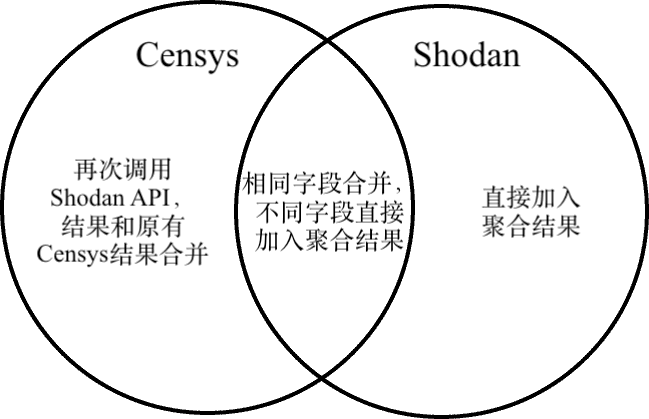
\includegraphics[scale=0.4]{merge.png}
    \caption{Censys和Shodan搜索结果融合示意图}
    \label{fig:merge}
  \end{figure}

在融合完Censys和Shodan之后,得到了一个融合的结果,接下来再用这个结果和ZoomEye进行融合。
和前述的方法一样,对于相同的IP地址的主机,相同字段合并,不同字段直接加入结果,不同IP的主机,
再去搜索另一方的API。不过,和上面的一样,考虑到Censys的速度和结果,只重新搜索了Shodan和ZoomEye。此外,和上述有一定区别是,
对于相同IP的主机进行结果合并时,把相同意义但是不同名字的字段只留下了一方的,比如Shodan的“location”字段和ZoomEye的“geoinfo”字段,
由于Shodan的“location”字段的信息更加具体,因此在合并时删除了ZoomEye的“geoinfo”字段,避免产生其他问题。

此外,在融合的时候,对每个结果添加了一个“source”字段,表示该主机的信息来自哪个API。
比如“Censys/Shodan/ZoomEye”就表示该主机的信息同时来自三个API,是这三者融合的结果,而如果只有两个,
就表示在另外一个API里面不存在该主机的信息。这样做可以在出现问题的时候重新去查找该API的原始信息,方便开发者定位错误,也方便了用户使用。

在三者的结果融合之后,把融合后的每一台主机的信息存储进入数据库,只有融合后的数据才是存储的对象,而融合前的数据不是。

\section{分析威胁情报的方法}
\label{chap3:analysis-strategy}

\subsection{对比中存在的问题}
\label{sec:comparation-problems}

在获得了详尽的主机信息和CVE信息之后,下一步就是对比主机上的信息和CVE的信息得到主机上可能存在的威胁。正如前面所述,
本文采用的方法是通过对比主机上的开放端口和CVE的可能产生威胁的端口,和主机上安装的软件和CVE的可能产生威胁的软件。
但是,在实际观察了主机上安装的软件的名称和版本和CVE的软件名称和版本后,发现软件名称会有多种叫法,比如“Tomcat”和“Apache Tomcat”;
版本也会存在多种叫法,比如“1.1.1a”和“1.1.1-log”。因此,如果仅简单使用字符串匹配的方式,很难对比出软件名称和版本是否相同。

此外,不论是对比成功的CVE还是由Shodan提供的CVE,其中都有大量的难以利用的CVE,它们的CVSS评分很低,如果也计入系统,
会让用户觉得系统里竟然有这么多的漏洞,从而产生困扰。

\subsection{对比端口和软件的策略}
\label{sec:comparation-strategy}

本小节介绍对于一台主机的信息,如何和一个CVE的信息进行对比,找到其上的可能的威胁端口和软件。

在对比操作中,首先需要找到安装在主机上的全部的开放端口和全部软件。端口方面,Shodan提供了“ports”字段,Censys也提供了“protocol”字段,
提取这两个中的信息即可获得全部开放端口。软件方面,遍历Shodan提供的“data”字段找到所有服务中运行的软件,和ZoomEye中分类好的所有软件信息,
即可获得所有的软件信息。

在对比端口的时候,直接把主机开放端口和CVE中提供的端口取交集,然后再去除其中的诸如80和443这样的常见端口即可,
因为这样的端口开放只能证明主机上运行了HTTP服务或者HTTPS服务,这样的主机非常多,如果判断它们都有可能受到威胁的话是不正确的。
相反,有一些不常见的端口却能代表一些软件的使用,比如4786,是cisco的IOS软件的默认端口,通过该端口的开放即可判断出该主机上运行了该软件。
在这种情况下,可以用该端口开放来判断主机有可能受到该CVE的威胁。

接着是判断软件是否存在交集,遍历本机软件和CVE中记录的可能的威胁软件。在判断软件是否一样的时候,
宗旨是不放过相同的软件但是并不要求完全排除不相同的软件也被当成相同的情况,于是采取一种折中的办法,也就是计分的方法。
对软件名称和软件版本分别对比,然后通过一种规则打分,超过一定值就判断两个软件可能一样。在给软件名称打分的时候,
应用的方法是求主机软件名称和CVE上提供的软件名称的最长公共子串长度占两者平均长度的比例的方法。
选用二者平均长度的原因是如果只选取一个长的就会出现比例总是很小的情况,而另一个长的只是在前面加上了供应商的名字;
而如果选取短的那个,就会出现如果其中一个软件的名称只有两三个字母直接被另一个包含的情况,这样比例直接为1,只选择其中一个名字也会有相同的问题,影响了准确性。

最长公共子串是一种基于动态规划的算法,它的目的是寻找两个字符串中最长的公共的子串的算法,
这里称为子串的原因是在两个母串中相同的字母必须是相同顺序并且连续。如“abcdefg”和“0bcde123g”的最长子串就是“bcde”,长度为4,
而子序列“bcdeg”因为“g”没有和“bcde”连续,因此并不能算是最长子串。

该算法的思路是,令两个母串分别为$s_1$和$s_2$,再令二维数组$c$,
而$c[i][j]$的含义是母串$s_1$的子串取到母串的第$i$个字符和母串$s_2$的子串取到母串的第$j$个字符时,
这两个母串的子串的最长公共子串的长度。因此,如果$s_1 [i]=s_2 [j]$,
则相当于每个母串的子串都褪掉各自的最后一个字符之后两个新的母串的子串再求最长公共子串的长度加一;如果不等,
则各自再尝试褪掉最后一个字符后分别和原来的对方母串求最长公共子串再求二者最大值。于是我们可以得到状态转移方程~\ref{equ:LCS}:

\begin{equation}
    \label{equ:LCS}
    c[i][j]=\begin{cases}
    0 & i=0 \, and \, j=0 \\
    c[i-1][j-1]+1 & s_1[i]=s_2[j] \\
    max(c[i-1][j], c[i][j-1]) & \text{else}
    \end{cases}
\end{equation}

判断软件版本是否相同方法是,先去掉二者中的非点和数字的字符,然后按照点进行分割,从前往后比较,每次相同则加上一定分数,
而越往后分数越高,意味着软件相同的可能性越来越高。

最后,把软件名称的分数和软件版本的分数相加,如果超过一个设定的阈值,则认为两个软件相同。

不过,这里还有一个问题,就是明明不是同一个软件,但是却有相同的软件版本,导致判断软件相同;或者虽然是同一个软件,但因为软件名称完全一样,
直接超过了设定的阈值,软件版本相差甚远却认为一样。因此,在首先计算完软件名称的分数之后,如果分数很低,就说明这一定不是相同软件,
直接认为两个软件不同;如果分数很高以至于接近1,就说明很有可能是相同软件,这时把阈值提高,让它再计算软件版本的分数后判断是否超过新的阈值。

对于一台主机来说,如果没有找到任何的可能的威胁端口和软件,则认为该主机不受该CVE威胁。

图~\ref{fig:comparation}是对于一台主机和一个CVE进行对比时的流程图。

\begin{figure}[H]
    \centering
    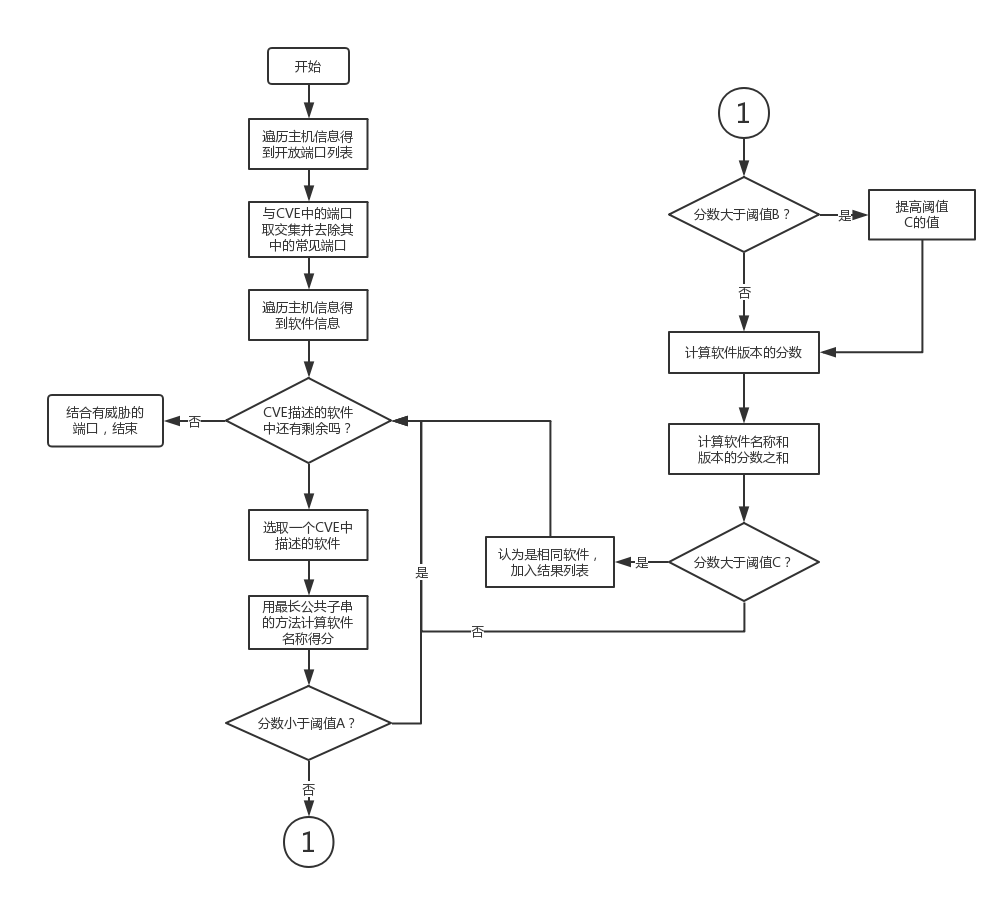
\includegraphics[scale=0.35]{comparation.png}
    \caption{一台主机和一个CVE进行对比时的流程图}
    \label{fig:comparation}
\end{figure}

\section{获取检测脚本的方法}
\label{sec:scripts}

获取检测脚本的目的是当系统提供给用户某主机存在某可能的威胁时,用户通过阅读CVE的介绍并不能清楚地判断该主机是否真的受到这个威胁,
这是就需要实际运行脚本来判断。而这种判断方法和渗透测试类似,也具有一定不可预测性,可能对主机产生不良的后果。在整个系统中,
处于爬取CVE相关信息的步骤,在爬取CVE Details网站的时候,也会一并找到检测的脚本。

正如~\ref{sec:Exploit-Database}节中介绍的一样,Exploit Database是一个漏洞利用脚本的数据库,它也提供了一个网站,展示了各种的利用脚本,
而每个脚本都对应了一个CVE。虽然如此,但是无法直接运行这些脚本来判断主机是否存在该漏洞,因为这些脚本语言不同,运行方法不同,
有的甚至存在bug无法运行,或者只是一句话让读者自己写代码实现。因此,只需要记录脚本地址然后附到CVE信息里即可。

然而,Exploit Database也没有提供API,不能直接找到脚本;也不支持爬虫,在爬取该网站的时候有人机检测,无法使用代码直接访问网站。
因此,本文使用了第三方搜索引擎来实现找到检测脚本的方法。这里选用的第三方搜索引擎是Google。在尝试了许多常见的搜索引擎之后,
发现只有Google能最准确地找到脚本。

具体的方法是在Google上搜索“\{CVE名称\} site:exploit-db.com”,这样搜索出来的结果就都来自于Exploit Database。
然后再判断Google给出的结果是否真的是正确的。一般来说只要再访问结果中提供的网址即可,但是Exploit Database不仅限制了非正常访问,
连单次代码访问都是禁止的。于是本文读取了Google返回的摘要信息,看里面是否存在完整的CVE名称,如果存在则结果正确,反之则不然。

然而,在实际操作中发现了一些问题,也即Google的访问问题,不论是Python上的Google Search的模块还是直接用爬虫访问Google的网站,
亦或用其他代理的Google,都无法长时间正常地使用,因此在实际系统中并没有加入这一部分,但是代码在该项目的代码仓库中存在。
